%
% File acl2017.tex
%
%% Based on the style files for ACL-2015, with some improvements
%%  taken from the NAACL-2016 style
%% Based on the style files for ACL-2014, which were, in turn,
%% based on ACL-2013, ACL-2012, ACL-2011, ACL-2010, ACL-IJCNLP-2009,
%% EACL-2009, IJCNLP-2008...
%% Based on the style files for EACL 2006 by 
%%e.agirre@ehu.es or Sergi.Balari@uab.es
%% and that of ACL 08 by Joakim Nivre and Noah Smith

\documentclass[11pt,a4paper]{article}
\usepackage[hyperref]{acl2017}
\usepackage{times}
\usepackage{latexsym}

%for the table
\usepackage{booktabs}

%for [H]
\usepackage{float}
\usepackage{graphicx}

\usepackage{url}

\aclfinalcopy % Uncomment this line for the final submission
%\def\aclpaperid{***} %  Enter the acl Paper ID here

%\setlength\titlebox{5cm}
% You can expand the titlebox if you need extra space
% to show all the authors. Please do not make the titlebox
% smaller than 5cm (the original size); we will check this
% in the camera-ready version and ask you to change it back.

\newcommand\BibTeX{B{\sc ib}\TeX}

\title{Evaluation of Neural Net Based Classifiers for Multi-Class Emoji Prediction}

\author{Yun Zhang \\
	 104946985 \\
	% \\
	 \\
	\small{\tt zhangmike@ucla.edu } \\\And
	Peter Kim \\
	204271299 \\
%	 \\
	 \\
	\small{\tt peterkim95@ucla.edu} \\\And
	Haoxiang Zhang \\
	104278461 \\
	% \\
	 \\
	\small{\tt zhanghaoxiang@ucla.edu} \\\And
	 Jonathan Hurwitz \\
	 804258351 \\
%	 \\
	 \\
	\small{\tt jdhurwitz@ucla.edu} \\
}
\date{}

\begin{document}
	\maketitle
	\begin{abstract}
		Modern users spend more and more time on social networking services (SNS), such as Twitter and Instagram. Huge amounts of data are generated at a surprisingly rapid speed. Across all popular social networking platforms, Emojis are used in addition to basic text. These provide an additional layer of meaning to the textual data, and can even be considered as pictorial summarizations of the text. Inspired by this idea, we want to create out a robust model to extract useful patterns from the data, explore the underlying relationship between Emojis and text, and predict the most likely Emoji(s) given an associated text. We will explore multiple the simple feed-forward neural network to get an idea of baseline performance before moving on towards the evaluation and design of more complicated models, such as GRU, Bi-GRU, LSTM, and Bi-LSTM.
	\end{abstract}
	
	\section{Introduction}
	
	The emoji prediction project is being hosted as a competition on codalab. The data consists of 500k tweets in English and 100k tweets in Spanish. We’ve focused on emoji prediction for English. Tweet dates span the range from October 2015 to February 2017 and are geolocalized to the US and Spain. The dataset was built from tweets that contain one and only one of the twenty most frequent emojis. The label set consists of the twenty most frequent emojis labeled numerically from 0-19.
	
	\begin{figure}[H]
		\hspace*{-1.3cm}
		\centering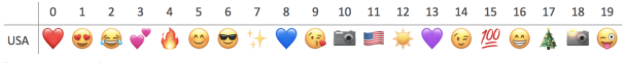
\includegraphics[scale=0.36]{emojis} 
		\caption{\textbf{ Mapping from emojis to numerical values.}}
	\end{figure}
	
	
	Our approach focused on evaluating several neural network architectures, starting with the simplest single-layer feed-forward model and extending to bidirectional RNN-based models. 
	
	
	\section{Models}
	
	\subsection{Feed Forward Neural Net}
	Since this is a multi-class classification problem, the basic neural net structure is aptly suited. Multi-class classification can be performed by increasing the number of nodes on the output layer to suit the dimension of the class vector. A function such as softmax can compress these values into a probabilistic range such that the sum of outputs for some input instance is 1. The feed-forward neural net, or multi-layer perceptron (MLP) model was meant to serve as a rough baseline for the project.
	\par
	Word embeddings were done by taking Google’s pretrained news vectors and performing mean aggregation on each tweet to create a tweet vector. Google’s model includes word vectors for a vocabulary of 3 million words and phrases, trained on 100 billion words from Google News. Each vector has dimension 300. The preprocessing step for the MLP model involves pulling all the tweets and tokenizing them. Unlike the preprocessing for later models discussed, the tokenization did not involve removing any words and was simply to split up a tweet’s word sequence into a list of words. A word embedding matrix was created by scanning through each tweet in the dataset, and for each word within the tweet, checking to see if the Google word2vec model had a vector representation for the word. If so, this vector became the representation of the word. If no occurence in the model, a zero-padded vector (of dimension 300) served as the representation. At the end of the sequence, the mean of these vectors was calculated as the corresponding “tweet” vector embedding. This final embedding was the input for the model.
	\par
	The MLP invariants included a 300-node input layer (one for each dimension) as well as a 20-node output layer, corresponding to a one-to-one mapping for the class assignments. Several experiments were done to test the effects of hidden layer node number as well as number of hidden layers. Due to time constraints, a full cross-validation and hyper parameter tuning exercise was not performed. 
	\par
	One criticism of MLP for sentiment analysis is the simplicity of the model in that it can’t encapsulate long-chain dependencies. There is no notion of a sequence and each data instance exists on its own. Tweets are sufficiently short (due to character limit) such that long-chain dependencies might not necessarily appear, but the more complicated models tested have been historically shown to model such dependencies successfully. 
	
	
	
	
	\subsection{Gated Recurrent Unit (GRU)}
	A recurrent neural network (RNN) is a class of neural network that has connections between units. Unlike feed-forward neural network, RNN has a memory to capture information that has already been calculated. This feature allows RNN to process arbitrary sequences of inputs. Gated recurrent unit (GRU) is a gating mechanism in RNN. Basically, a GRU has a reset gate and an update gate. The reset gate combines the new input with the previous memory, and the update gate decides how much of the previous memory should be kept. The GRU model serves as one of more complicated models that should be more accurate than our baseline MLP model.
	\begin{figure}[H]
		\hspace*{-1.3cm}
		\centering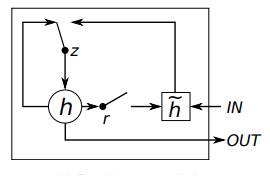
\includegraphics[scale=0.7]{gru} 
		\caption{\textbf{ GRU. Chung, Junyoung, et al. “Empirical evaluation of gated recurrent neural networks on sequence modeling.” (2014).}}
	\end{figure}

	
	
	
	\subsection{Bidirectional Gated Recurrent Unit (Bi-GRU)}
	\label{sect:pdf}
	
	Besides the standard gated recurrent unit (GRU), we also implemented a bidirectional gated recurrent unit (Bi-GRU). Bi-GRU was used to increase the amount of information available to the recurrent neural network. By constructing neurons in both forward and backward directions, the current state of of Bi-GRU can obtain information from past and future states. This is extremely useful when understanding the context of input, especially for longer bodies of texts. However, since tweets are generally no more than 20 words, we expect that this bidirectional model will have a marginal performance gain over the previous GRU model.
	

	
	\subsection{Long Short Term Memory (LSTM)}
	
	The LSTM introduces the concept of a memory cell, consisting of four main elements: an input gate, a neuron with a path back to itself, a forget gate, and an output gate. The loop back allows the state of a memory cell to remain constant through time. The forget gate modulates the loop back and can allow the cell to “delete” or “forget” its previous state. LSTMs do not suffer from the vanishing or exploding gradient problem when long sequences are processed. It is an effective model for data that exhibits long-chain dependencies. We expect that this model will perform similarly to the GRU model, but will take longer to train as LSTMs are more computationally expensive than GRUs.  
	 \begin{figure}[H]
	 	\hspace*{-1.3cm}
	 	\centering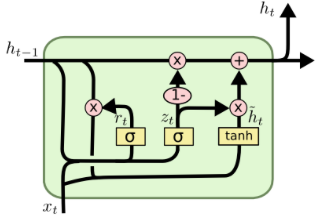
\includegraphics[scale=0.7]{lstm_image} 
	 	\caption{\textbf{ The LSTM model, showing flow of information and gating.}}
	 \end{figure}
	
	\begin{figure}[H]
		\hspace*{-1.3cm}
		\centering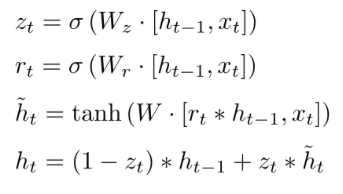
\includegraphics[scale=0.5]{lstm_functions} 
		\caption{\textbf{ LSTM functions.}}
	\end{figure}
	\subsection{Bidirectional Long Short Term Memory (Bi-LSTM)}
	LSTMs only preserve past information because inputs that have been seen are from the past. A bidirectional model allows the inputs to run in the positive and negative direction, at the same time. This is essentially like getting a past view and future view of information. With a bidirectional LSTM, at any point in time you can preserve information from both past and future information.
	
\section{Results}

For evaluation, we used accuracy as well as the F1 score, which is a harmonic mean of precision and recall. The task is evaluated based on Macro F-score, as the fundamental idea of this task is to encourage systems to perform well overall, which would inherently mean a better sensitivity to the use of emojis in general, rather than for instance overfitting a model to do well in the  three or four most common emojis of the test data. Macro F-score can be defined as simply the average of the individual label-wise F-scores.

\par
To generate large training dataset, we used Tweepy to crawl about 480,000 tweets with exactly one emoji among the top 20 emojis in English tweets. After training our models on this body of tweets, we tested on the trial dataset provided by the competition hosts, which contains 50,000 tweets. We build a vocabulary based on the training dataset and use <UNK> for unknown words at test time. After word embeddings, the input to our models are concatenations of 300-dimensional word-embedding vectors. We chose word embedding size d = 300, and use the 300 dimensional pre-trained GloVe word embeddings. The dimension of the hidden layer is 200 and the output size is 20 according to 20 labels we need to predict from. In addition, we use a mini-batch size of 32, set the learning rate at 1e-4 and train the model for 500 epochs.	

\subsection{Comparison of Model Accuracy and F1}
The table below shows a comparison of the F1-scores and dev accuracies for each of the five models. The feed-forward neural net, or multi-layer perceptron (MLP) performed the best with a dev accuracy of 73.9\%, and an F1-score of 58.2. The fact that the F1-score is much lower than accuracy might indicate that this model is predicting the most common emojis rather than encapsulating information inherent in the text that lends itself to accurate predictions.
	\begin{table}[htp]
		\centering
		\caption{F1-Score and Accuracy for Dev Set}
		\label{my-label}
		\begin{tabular}{@{}lll@{}}
			\toprule
			Model       & F1-Score & Dev Accuracy \\ \midrule
			FF NN (MLP) & 58.2     & 73.9         \\
			GRU         & 45.6     & 45.9         \\
			Bi-GRU      & ?        & ?            \\
			LSTM        & 44.3     & 45.1         \\
			Bi-LSTM     & ?        & ?            \\ \bottomrule
		\end{tabular}
	\end{table}
%	\section*{Acknowledgments}

\subsection{Discussion}
	The FF NN model performed significantly better than our RNN models. We believe this is because the sequences in tweets are too short, and therefore does not capture any useful sequential information. Also, emojis are usually dependent on only a single word in a tweet and not the whole semantic meaning of the tweet. Therefore, the sequence information captured by RNNs in general could be ultimately unhelpful for predicting the emoji used.
	\par
	The hypothesis that an emoji is dependent on the word and not the sequence of words is further strengthened by the following observation: there was a severe performance drop (~20\%) when we use a low dimensional word embedding (d = 50). Here, we realize that using a lower dimensional embedding loses information of each word and semantic meaning between words. This meaning, we hypothesize, is the most critical aspect to correctly predicting an emoji.
	\par
	As hypothesized, both the GRU and LSTM models performed very similarly, and the LSTM model took ~10 minutes more for training a single epoch. 
	
\section{Conclusion}
	In this report, we examined several different neural network models to help us predict an emoji given a tweet. The one that performed best was the simplest model: the FF NN model. It achieved state-of-the-art results as it sits at second place on the official CodaLab leaderboards. Overall, we think the RNN models are still valuable models that helped us demonstrate our understanding of common NLP techniques in deep learning.
	
	\section{References}
	Eisner, Ben, et al. "emoji2vec: Learning emoji representations from their description." arXiv preprint arXiv:1609.08359 (2016).
	\newline
		\newline
	Zhao, Luda, and Connie Zeng. "Using Neural Networks to Predict Emoji Usage from Twitter Data."
		\newline
		\newline
	Hallsmar, Fredrik, and Jonas Palm. "Multi-class sentiment classification on twitter using an emoji training heuristic." (2016).
		\newline
		\newline
	Barbieri, Francesco, Francesco Ronzano, and Horacio Saggion. "What does this Emoji Mean? A Vector Space Skip-Gram Model for Twitter Emojis." LREC. 2016.
		\newline
		\newline
	Barbieri, Francesco, et al. "How cosmopolitan are emojis?: Exploring emojis usage and meaning over different languages with distributional semantics." Proceedings of the 2016 ACM on Multimedia Conference. ACM, 2016.
		\newline
		\newline
	Espinosa-Anke, Luis, Horacio Saggion, and Francesco Barbieri. "Revealing patterns of Twitter emoji usage in Barcelona and Madrid." Frontiers in Artificial Intelligence and Applications. 2016;(Artificial Intelligence Research and Development) 288: 239-44.(2016).
		\newline
		\newline
	Sampietro, Agnese. "EXPLORING THE PUNCTUATING EFFECT OF EMOJI IN SPANISH WHATSAPP CHATS." Lenguas Modernas 47 (2016).
		\newline
		\newline
	Barbieri, Francesco, Miguel Ballesteros, and Horacio Saggion. "Are Emojis Predictable?." arXiv preprint arXiv:1702.07285(2017).
	
	% include your own bib file like this:
	%\bibliographystyle{acl}
	%\bibliography{acl2017}
%	\bibliography{biblio}
%	\bibliographystyle{acl}
	
	\appendix
	
	
	
\end{document}
